\begin{frame}{Quantum Computing: New Paradigm for Computation}
  Quantum computing uses specialized {\color{red}quantum technology} to solve {\color{red}complex problems}
  that classical computers cannot solve {\color{red}quickly enough}.

 \begin{figure}
    \centering
    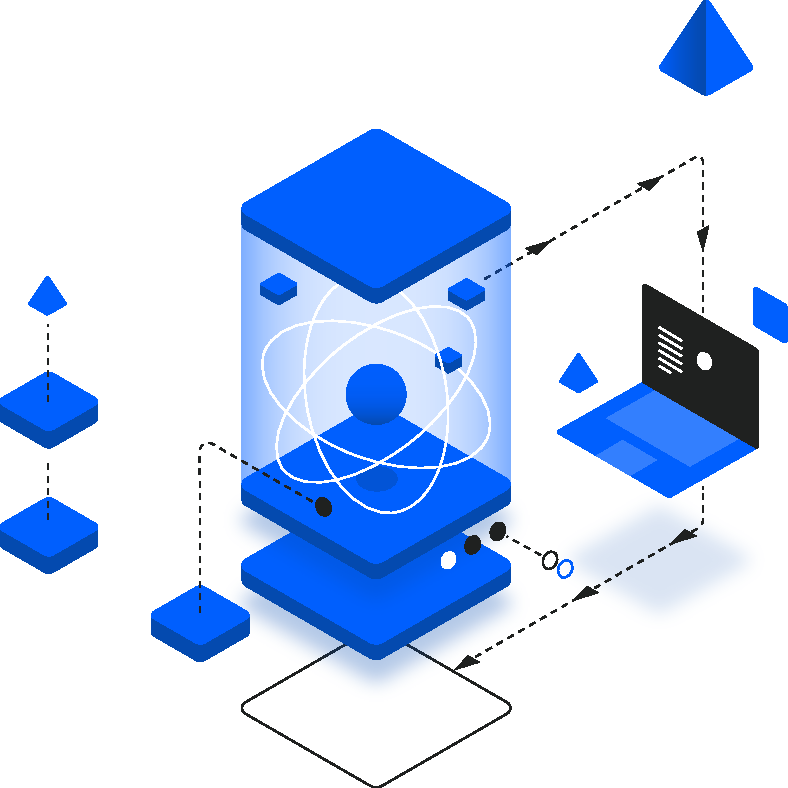
\includegraphics[width=0.5\linewidth]{quantum_computing_schematic.pdf}
    \caption*{Credit: PSNC}
  \end{figure}
\end{frame}


\begin{frame}{Examples of Complex Problems}
    Quantum Chemistry, Electronic Structure of Molecular Systems.
    \begin{figure}
      \def\range{8}
      \def\xyRatio{2/3}
      \def\circSize{1mm}
      \centering
      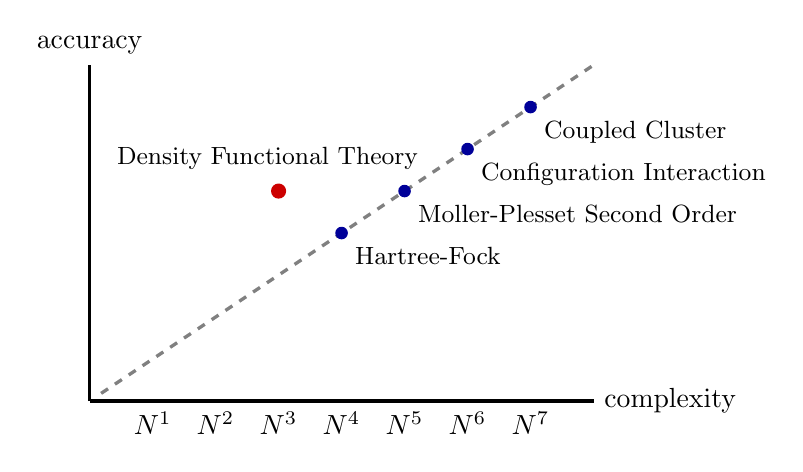
\begin{tikzpicture}[-, very thick, align=center, scale=0.8]
        \draw (0,0) -- (0,\range*\xyRatio) node[above] {accuracy};
        \draw (0,0) -- (\range,0) node[right] {complexity};
        \foreach \n in {1,...,7}
        \node[below] at (\n,0) {$N^\n$};

        \draw[dashed, gray, shorten <=5] (0,0) -- (\range,\range*\xyRatio);

        \foreach \n/\name/\abbr in {4/Hartree-Fock/HF, 5/Moller-Plesset Second Order/MP2, 6/Configuration Interaction/CISD, 7/Coupled Cluster/CCSD(T)}
        \fill[blue!60!black] (\n,\xyRatio*\n) circle (\circSize)
        node[align=left, below right=1pt, black] (\abbr) {\small\name};

        % \draw[red, thick] (HF) -- (SE);

        \fill[red!80!black] (3,5*\xyRatio) circle (1.2*\circSize) node[above=4pt, xshift=-4pt, black] (DFT) {\small Density Functional Theory};
        % \fill[blue!60!black] (4.5,6.5*\xyRatio) circle (\circSize) node[left=1ex, black] {Deep QMC};
      \end{tikzpicture}
      \caption*{Credit: Janosh Riebesell}
    \end{figure}

\end{frame}

\begin{frame}{Examples of Complex Problems}
    Discrete logarithm, Prime factorization in cryptography.
    \begin{figure}
      \centering
      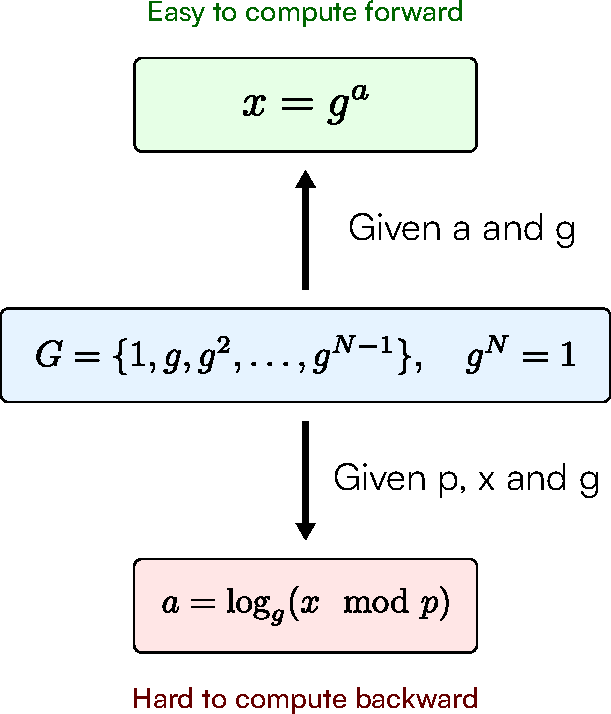
\includegraphics[width=0.5\linewidth]{discrete_logarithm_problem.pdf}
      \caption*{Credit: Anthropic's Claude Sonnet 3.5 LLM}
    \end{figure}
\end{frame}

\begin{frame}{Quantum Computing Hardware Since 2016}
  \begin{itemize}
    \setlength\itemsep{0.1em}
    \item The first generally available cloud-based quantum processor had {\color{red}5 quantum bits, or qubits}:
  \end{itemize}

  \begin{figure}
    \centering
    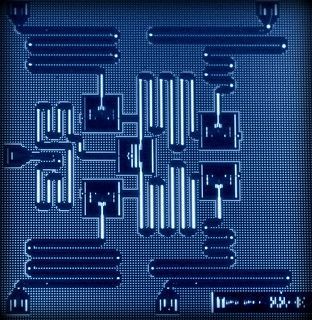
\includegraphics[width=0.3\linewidth]{5q_transmon.jpg}
    \vspace*{-3mm}
    \caption*{Credit: IBM}
  \end{figure}

  \begin{itemize}
    \setlength\itemsep{0.1em}
     \item Use cases limited to proof-of-concept demonstrations:
  \end{itemize}

  \begin{figure}
    \centering
    
\includegraphics[width=1.0\linewidth]{yours_truly.png}
  \end{figure}
\end{frame}

\begin{frame}{Scaling Up Quantum Computing Hardware}
  Generally available state-of-the-art devices can have as many as {\color{red}433} noisy qubits.

  \begin{figure}
    \centering
    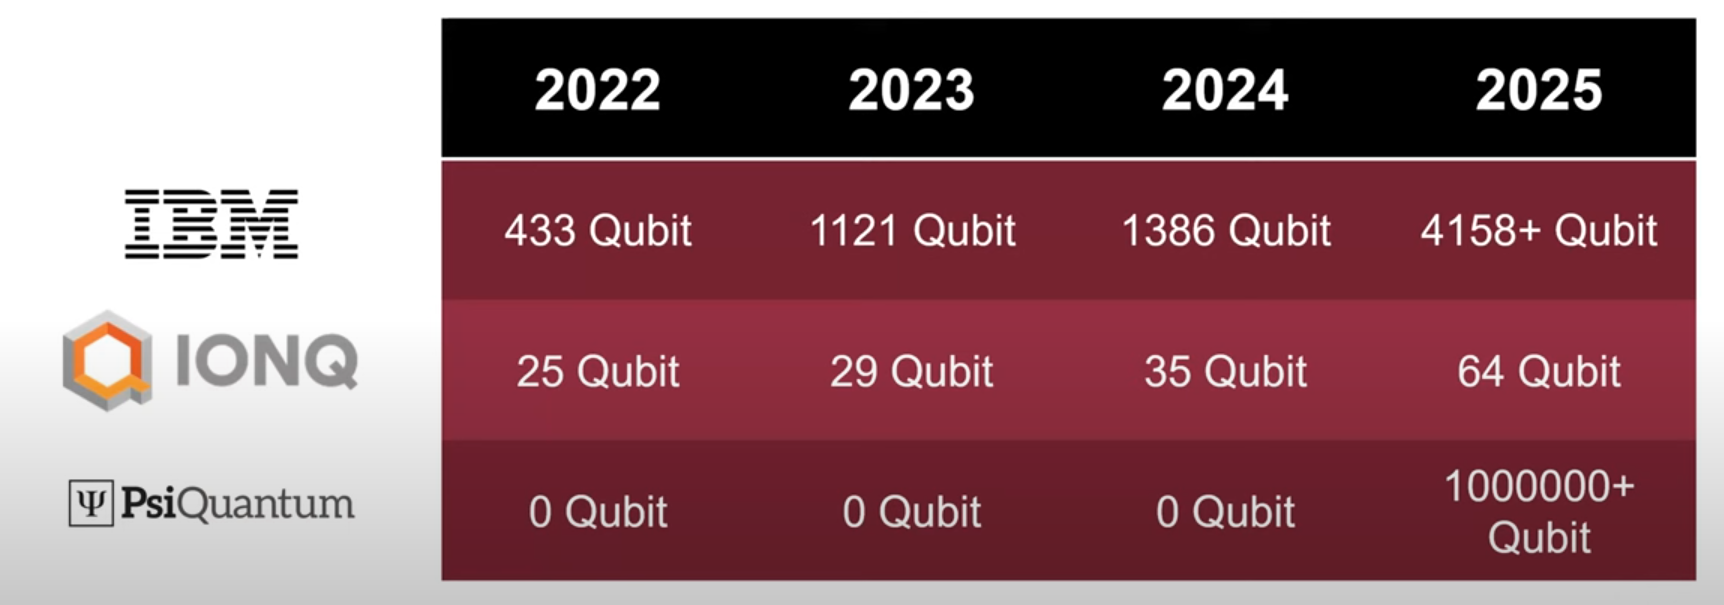
\includegraphics[width=1.0\linewidth]{projections.png}
    \caption*{Credit: Tobias Osborne}
  \end{figure}
  Despite increasing qubit numbers, {\color{red}Quantum Advantage} is yet to be realized.
\end{frame}
